% Copyright 2007 by Till Tantau
%
% This file may be distributed and/or modified
%
% 1. under the LaTeX Project Public License and/or
% 2. under the GNU Public License.
%
% See the file doc/licenses/LICENSE for more details.

\documentclass[portuguese,10pt,xcolor=table]{bredelebeamer}
\setbeameroption{show notes}

\usepackage[brazil]{babel}
\usepackage[utf8]{inputenc}
\usepackage{times}
\usepackage{varwidth}
\usepackage{tikz}
\usepackage{pifont}
\usepackage{tikzsymbols}
\usepackage{listings} % Código de programas
%\usepackage[tikz]{bclogo}
\usetikzlibrary{arrows,shapes}

\usetikzlibrary{calc,decorations.pathmorphing,patterns}
\pgfdeclaredecoration{penciline}{initial}{
	\state{initial}[width=+\pgfdecoratedinputsegmentremainingdistance,
		auto corner on length=1mm,]{
			\pgfpathcurveto%
			{% From
				\pgfqpoint{\pgfdecoratedinputsegmentremainingdistance}
				{\pgfdecorationsegmentamplitude}
			}
			{%  Control 1
				\pgfmathrand
					\pgfpointadd{\pgfqpoint{\pgfdecoratedinputsegmentremainingdistance}{0pt}}
				{\pgfqpoint{-\pgfdecorationsegmentaspect
							   \pgfdecoratedinputsegmentremainingdistance}%
							   {\pgfmathresult\pgfdecorationsegmentamplitude}
				}
			}
			{%TO 
				\pgfpointadd{\pgfpointdecoratedinputsegmentlast}{\pgfpoint{1pt}{1pt}}
			}
		}
	\state{final}{}
}


\lstset{
	language=C,
	%basicstyle=\footnotesize\ttfamily,
	basicstyle=\normalsize\ttfamily,
	%keywordstyle=\footnotesize\bfseries\sffamily,
	keywordstyle=\scriptsize\bfseries\sffamily,
	showstringspaces=false,
	numbers=left,
	numberstyle=\scriptsize,
	stepnumber=1,
	numbersep=29pt,
	%backgroundcolor=\color{blue!05},
	backgroundcolor=\color{gray!35},
	keywordstyle=\bfseries\color{green!40!black},
	commentstyle=\itshape\color{purple!40!black},
	identifierstyle=\color{blue},
	stringstyle=\color{red},
	extendedchars=true,
	commentstyle=\color{green!40!black}
	showspaces=false,
	showtabs=false,
	}
	\renewcommand{\lstlistingname}{Código}

\everymath{\displaystyle}
\tikzstyle{every picture}+=[remember picture,decoration=penciline]
\DeclareTextFontCommand{\textdf}{\bfseries\color{blue!80}}
%\tikzstyle{every node}+=[decorate]
%\tikzstyle{every path}+=[decorate]
%\tikzstyle{na} = [baseline=-.5ex]

\usepackage[T1]{fontenc}

\def\lecturename{IMD0012 - Introdução às técnicas de programação}

\title{\insertlecture}

\author{Prof. Fernando Figueira\\(adaptado do material do Prof. Rafael Beserra Gomes)}

\institute{UFRN}

\subject{Ponteiros e Alocação Dinâmica}

\lecture[]{Ponteiros e Alocação Dinâmica}{}

\subtitle{Introdução}

\date{}

\begin{document}

\usebackgroundtemplate{%
	
\includegraphics[width=\paperwidth,height=\paperheight]{background2}
}
\begin{frame}
  \maketitle
 \begin{center}
 \tiny
Material compilado em \today.\\
  Licença desta apresentação:\\
		
\includegraphics[height=1.0cm]{by-nc-nd.png}\\
http://creativecommons.org/licenses/
	\end{center}
\end{frame}

	\def\GN[#1]{\colorbox{gray!40}{#1}}
	\def\RN[#1]{\colorbox{red!40}{#1}}
	\def\BN[#1]{\colorbox{blue!40}{#1}}
	\def\RBN[#1]{\cellcolor{blue!40}{ #1 }}
	\def\RON[#1]{\cellcolor{orange!40}{ #1 }}
	\def\ON[#1]{\colorbox{orange!40}{#1}}
	\def\WN[#1]{\colorbox{white!40}{#1}}
	\def\GZ[#1]{\colorbox{gray!40}{\textbf{#1}}}
	\def\BZ[#1]{\colorbox{blue!40}{\textbf{#1}}}

\section{Ponteiros}
	
	\begin{frame}
		\begin{center}
			\structure{\large Endereço base}
		\end{center}
	\end{frame} 

	\begin{frame}
		\tiny
		 \setlength{\tabcolsep}{0pt}	
		\begin{table}
				  \begin{tabular}{|@{\hskip 0.2cm}c@{\hskip 0.2cm}|c|c|c|c|c|c|c|c|@{\hskip 0.2cm}c@{\hskip 0.2cm}|}
					\hline
					0xbffff22c & \GN[0]&\GN[0]&\GN[0]&\GN[0]&\GN[0]&\GN[1]&\GN[0]&\GN[1]& \textbf{short int} a = 5\\\hline
		0xbffff22d & \BN[0]&\BN[1]&\BN[0]&\BN[0]&\BN[0]&\BN[0]&\BN[1]&\BN[0]& \textbf{char} b = 'B'\\\hline
		0xbffff22e & \BN[0]&\BN[1]&\BN[0]&\BN[0]&\BN[0]&\BN[0]&\BN[1]&\BN[1]& \textbf{char} x = 'C'\\\hline
		\tikz[overlay] \node[fill=blue!20,shape=rectangle,minimum width=1cm,minimum height=0.4cm,opacity=1.0](e4){0xbffff22f}; & \RN[1]&\RN[1]&\RN[0]&\RN[1]&\RN[1]&\RN[1]&\RN[0]&\RN[1]& \textbf{float} y = 3.2 \\\hline
		0xbffff230 & \RN[1]&\RN[1]&\RN[0]&\RN[0]&\RN[1]&\RN[1]&\RN[0]&\RN[0]& \\\hline
		0xbffff231 & \RN[0]&\RN[1]&\RN[0]&\RN[0]&\RN[1]&\RN[1]&\RN[0]&\RN[0]& \\\hline
		0xbffff232 & \RN[0]&\RN[1]&\RN[0]&\RN[0]&\RN[0]&\RN[0]&\RN[0]&\RN[0]& \\\hline
		0xbffff233 & \BN[0]&\BN[1]&\BN[0]&\BN[0]&\BN[0]&\BN[0]&\BN[0]&\BN[1]&  \textbf{char} t1 = 'A'\\\hline
		0xbffff234 & \BN[0]&\BN[1]&\BN[0]&\BN[0]&\BN[0]&\BN[0]&\BN[1]&\BN[0]& \textbf{char} t2 = 'B'\\\hline
		0xbffff235 & \BN[0]&\BN[1]&\BN[0]&\BN[0]&\BN[0]&\BN[0]&\BN[1]&\BN[1]& \textbf{char} t3 = 'C'\\\hline
		0xbffff236 & \BN[0]&\BN[1]&\BN[0]&\BN[0]&\BN[0]&\BN[0]&\BN[1]&\BN[1]& \textbf{char} t4 = 'A'\\\hline
		0xbffff237 & \GN[1]&\GN[1]&\GN[1]&\GN[1]&\GN[1]&\GN[0]&\GN[1]&\GN[1]& \textbf{short int} u = -5\\\hline
		0xbffff238 & \ON[0]&\ON[0]&\ON[0]&\ON[0]&\ON[0]&\ON[0]&\ON[0]&\ON[0]& \textbf{int} v = 1\\\hline
		0xbffff239 & \ON[0]&\ON[0]&\ON[0]&\ON[0]&\ON[0]&\ON[0]&\ON[0]&\ON[0]& \\\hline
		0xbffff23a & \ON[0]&\ON[0]&\ON[0]&\ON[0]&\ON[0]&\ON[0]&\ON[0]&\ON[0]& \\\hline
		0xbffff23b & \ON[0]&\ON[0]&\ON[0]&\ON[0]&\ON[0]&\ON[0]&\ON[0]&\ON[1]& \\\hline
				\end{tabular}
		\end{table}
		\tikz[overlay] \node[align=left,anchor=west,inner sep=4pt,fill=blue!20,opacity=0.8,rounded corners,scale=0.82,align=left](e9){\large \textbf{endereço base} da variável y};
		\tikz[overlay] \path[->,bend left] (e9.north) edge (e4.west);
		\normalsize
	\end{frame}


	\begin{frame}
		\begin{center}
			\structure{\large Ponteiros}
		\end{center}
	\end{frame} 

	\begin{frame} 
		\begin{beamerboxesrounded}{Definição}
			Uma variável que contém como valor um endereço de memória.
		\end{beamerboxesrounded}
		\vspace{0.4cm}
		A quantidade de bits necessária para representar um endereço de memória depende da arquitetura do computador e do sistema operacional. \\

	\end{frame}


	\begin{frame}
		\begin{center}
			\structure{\large Exemplo de ponteiro}
		\end{center}
	\end{frame} 

	\begin{frame}
		\tiny
		 \setlength{\tabcolsep}{0pt}	
		\begin{table}
				  \begin{tabular}{|@{\hskip 0.2cm}c@{\hskip 0.2cm}|c|c|c|c|c|c|c|c|@{\hskip 0.2cm}c@{\hskip 0.2cm}|}
					\hline
	\tikz[overlay] \node[fill=blue!20,shape=rectangle,minimum width=1cm,minimum height=0.4cm,opacity=1.0](e4){0xbffff22f};	& \RN[1]&\RN[1]&\RN[0]&\RN[1]&\RN[1]&\RN[1]&\RN[0]&\RN[1]& \textbf{float euro} = 4.075\\\hline
		 0xbffff230 & \RN[1]&\RN[1]&\RN[0]&\RN[0]&\RN[1]&\RN[1]&\RN[0]&\RN[0]& \\\hline
		0xbffff231 & \RN[0]&\RN[1]&\RN[0]&\RN[0]&\RN[1]&\RN[1]&\RN[0]&\RN[0]& \\\hline
		0xbffff232 & \RN[0]&\RN[1]&\RN[0]&\RN[0]&\RN[0]&\RN[0]&\RN[0]&\RN[0]& \\\hline
		0xbffff233 & \BN[0]&\BN[1]&\BN[0]&\BN[0]&\BN[0]&\BN[0]&\BN[0]&\BN[1]& \textbf{char t} = 'A'\\\hline
	\tikz[overlay] \node[fill=blue!20,shape=rectangle,minimum width=1cm,minimum height=0.4cm,opacity=1.0](e5){0xbffff234};	& \RN[1]&\RN[1]&\RN[0]&\RN[1]&\RN[1]&\RN[1]&\RN[0]&\RN[1]& \textbf{float dolar} = 3.305\\\hline
		 0xbffff235 & \RN[1]&\RN[1]&\RN[0]&\RN[0]&\RN[1]&\RN[1]&\RN[0]&\RN[0]& \\\hline
		0xbffff236 & \RN[0]&\RN[1]&\RN[0]&\RN[0]&\RN[1]&\RN[1]&\RN[0]&\RN[0]& \\\hline
		0xbffff237 & \RN[0]&\RN[1]&\RN[0]&\RN[0]&\RN[0]&\RN[0]&\RN[0]&\RN[0]& \\\hline
					0xbffff238 & \ON[1]&\ON[0]&\ON[1]&\ON[1]&\ON[1]&\ON[1]&\ON[1]&\ON[1]& \textbf{float * moedaPtr} =\tikz \node[fill=blue!20,shape=rectangle,minimum width=1cm,minimum height=0.2cm,opacity=1.0](e9){0xbffff22f};  \\\hline
		0xbffff239 & \ON[1]&\ON[1]&\ON[1]&\ON[1]&\ON[1]&\ON[1]&\ON[1]&\ON[1]& \\\hline
		0xbffff23A & \ON[1]&\ON[1]&\ON[1]&\ON[1]&\ON[0]&\ON[0]&\ON[1]&\ON[0]& \\\hline
		0xbffff23B & \ON[0]&\ON[0]&\ON[1]&\ON[0]&\ON[1]&\ON[1]&\ON[1]&\ON[1]& \\\hline

				\end{tabular}
		\end{table}
		\tikz[overlay] \path[->,bend right] (e9.north) edge (e4.east);
	\end{frame}


	\begin{frame}
		Ponteiro para char:
		\tiny
		 \setlength{\tabcolsep}{0pt}	
		\begin{table}
				  \begin{tabular}{|@{\hskip 0.2cm}c@{\hskip 0.2cm}|c|c|c|c|c|c|c|c|@{\hskip 0.2cm}c@{\hskip 0.2cm}|}
					\hline
		0xbffff22d & \BN[0]&\BN[1]&\BN[0]&\BN[0]&\BN[0]&\BN[0]&\BN[1]&\BN[0]& \textbf{char} b = 'B'\\\hline
		0xbffff22e & \BN[0]&\BN[1]&\BN[0]&\BN[0]&\BN[0]&\BN[0]&\BN[1]&\BN[1]& \textbf{char} x = 'C'\\\hline
	0xbffff22f	& \RN[1]&\RN[1]&\RN[0]&\RN[1]&\RN[1]&\RN[1]&\RN[0]&\RN[1]& \textbf{float} y = 3.2\\\hline
		 0xbffff230 & \RN[1]&\RN[1]&\RN[0]&\RN[0]&\RN[1]&\RN[1]&\RN[0]&\RN[0]& \\\hline
		0xbffff231 & \RN[0]&\RN[1]&\RN[0]&\RN[0]&\RN[1]&\RN[1]&\RN[0]&\RN[0]& \\\hline
		0xbffff232 & \RN[0]&\RN[1]&\RN[0]&\RN[0]&\RN[0]&\RN[0]&\RN[0]&\RN[0]& \\\hline
		0xbffff233 & \BN[0]&\BN[1]&\BN[0]&\BN[0]&\BN[0]&\BN[0]&\BN[0]&\BN[1]&  \textbf{char} t1 = 'A'\\\hline
		\tikz[overlay] \node[fill=blue!20,shape=rectangle,minimum width=1cm,minimum height=0.4cm,opacity=1.0](e4){0xbffff234};  & \BN[0]&\BN[1]&\BN[0]&\BN[0]&\BN[0]&\BN[0]&\BN[1]&\BN[0]& \textbf{char} t2 = 'B'\\\hline
		0xbffff235 & \BN[0]&\BN[1]&\BN[0]&\BN[0]&\BN[0]&\BN[0]&\BN[1]&\BN[1]& \textbf{char} t3 = 'C'\\\hline
		0xbffff236 & \BN[0]&\BN[1]&\BN[0]&\BN[0]&\BN[0]&\BN[0]&\BN[1]&\BN[1]& \textbf{char} t4 = 'A'\\\hline
		0xbffff237 & \GN[1]&\GN[1]&\GN[1]&\GN[1]&\GN[1]&\GN[0]&\GN[1]&\GN[1]& \textbf{short int} u = -5\\\hline
		0xbffff238 & \ON[1]&\ON[0]&\ON[1]&\ON[1]&\ON[1]&\ON[1]&\ON[1]&\ON[1]& \textbf{char *} p = \tikz \node[fill=blue!20,shape=rectangle,minimum width=1cm,minimum height=0.2cm,opacity=1.0](e9){0xbffff234};\\\hline
		0xbffff239 & \ON[1]&\ON[1]&\ON[1]&\ON[1]&\ON[1]&\ON[1]&\ON[1]&\ON[1]& \\\hline
		0xbffff23a & \ON[1]&\ON[1]&\ON[1]&\ON[1]&\ON[0]&\ON[0]&\ON[1]&\ON[0]& \\\hline
		0xbffff23b & \ON[0]&\ON[0]&\ON[1]&\ON[1]&\ON[0]&\ON[1]&\ON[0]&\ON[0]& \\\hline

				\end{tabular}
		\end{table}
		\tikz[overlay] \path[->,bend left] (e9.west) edge (e4.south);
		\normalsize
	\end{frame}


	\subsection{Implementação}

	\begin{frame}
		\begin{center}
			\structure{\large \insertsubsection}
		\end{center}
	\end{frame} 

	\begin{frame}
		\textbf{Declarando ponteiros:}\\
				\lstinputlisting{declaracao.c}
				\begin{itemize}
					\item \textbf{a} e \textbf{c}: tipo int
					\item \textbf{b}: \textbf{ponteiro para inteiro}
				\end{itemize}
	\end{frame}

	\begin{frame}
		\textbf{Atribuindo valores:}\\
				\lstinputlisting{atribuicao.c}
				\begin{itemize}
					\item é possível atribuir manualmente um endereço (não usual)
					\item operador \&: obtém o endereço da variável
		\end{itemize}
	\end{frame}

	
	\begin{frame}
		\textbf{Atribuindo valores:}\\
				\lstinputlisting{atribuicao3.c}
				\textdf{NULL}: o ponteiro não está armazenando um endereço válido
	
				\begin{itemize}
					\item bastante útil em estruturas de dados:
				\end{itemize}
						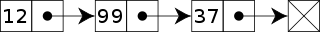
\includegraphics[height=0.5cm]{linkedlist.png}\\
	\end{frame}
	
	\begin{frame}
		\textbf{Escrevendo na tela o valor de um ponteiro:}\\
				\lstinputlisting{print.c}
				Use \%p no printf. Observe que é atribuído um endereço diferente a cada execução do programa.
	\end{frame}
	
	\begin{frame}
		\begin{alertblock}{\ding{46} Exercício em sala}
			\begin{enumerate}
				\item Declare dois inteiros: a e b (valores iniciais: 2 e 3)
				\item Declare três ponteiros para inteiro: p1, p2, p3
				\item Atribua NULL para p1
				\item Atribua o endereço de a para p2
				\item Atribua o endereço de b para p3
				\item Escreva na tela duas vezes o endereço de a: usando o operador \& e usando o valor do ponteiro
				\item Escreva na tela duas vezes o endereço de b: usando o operador \& e usando o valor do ponteiro
			\end{enumerate}
		\end{alertblock}
	\end{frame}
	
	\begin{frame}
		\begin{alertblock}{\ding{46} Exercício em sala}
			Atribua um valor ao ponteiro p de forma que o printf escreva somente \textbf{"uma string com varias palavras"}.
				\lstinputlisting{exercicio1.c}
		\end{alertblock}
	\end{frame}

	\section{Derreferenciação}
	\begin{frame}
		\textbf{Derreferenciando um ponteiro:}\\
				\lstinputlisting{derreferenciar.c}
				\textdf{Derreferenciar} um ponteiro: obter o valor no endereço de memória armazenado no ponteiro\\
				\textdf{Uso:} operador * antes do ponteiro.
				\begin{center}
	\end{center}
	\end{frame}

	\section{Aritmética de ponteiros}
	\begin{frame}
		\begin{center}
			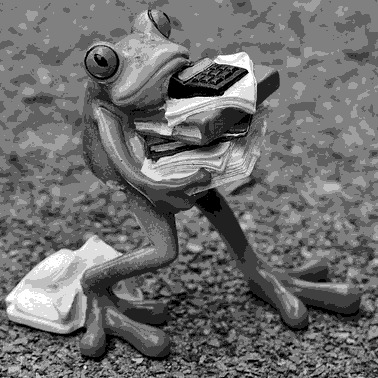
\includegraphics[height=4cm]{frog.jpg}\\
			\Large Aritmética de ponteiros
		\end{center}
	\end{frame}

	\begin{frame}
		\textbf{Aritmética de ponteiros:}\\
		\tiny
		Suponha um vetor declarado como: \textbf{int x[4];}
		 \setlength{\tabcolsep}{0pt}	
		 \begin{columns}[t]
			 \begin{column}[T]{.6\textwidth}
				 \begin{table}
		\scriptsize
					 \begin{tabular}{|@{\hskip 0.2cm}c@{\hskip 0.2cm}|c|c|c|c|c|c|c|c|@{\hskip 0.2cm}c@{\hskip 0.2cm}|}
						 \hline
						 \tikz \node[fill=blue!20,shape=rectangle,minimum width=1cm,minimum height=0.2cm,opacity=1.0](e4){0xbffff228}; & \RBN[0]&\RBN[0]&\RBN[0]&\RBN[0]&\RBN[0]&\RBN[0]&\RBN[0]&\RBN[0]& \textbf{x[0]} = 15\\\hline
						 0xbffff229 & \RBN[0]&\RBN[0]&\RBN[0]&\RBN[0]&\RBN[0]&\RBN[0]&\RBN[0]&\RBN[0]& \\\hline
						 0xbffff22a & \RBN[0]&\RBN[0]&\RBN[0]&\RBN[0]&\RBN[0]&\RBN[0]&\RBN[0]&\RBN[0]& \\\hline
						 0xbffff22b & \RBN[0]&\RBN[0]&\RBN[0]&\RBN[0]&\RBN[1]&\RBN[1]&\RBN[1]&\RBN[1]& \\\hline
						 0xbffff22c & \RBN[0]&\RBN[0]&\RBN[0]&\RBN[0]&\RBN[0]&\RBN[0]&\RBN[0]&\RBN[0]& \textbf{x[1]} = 10\\\hline
						 0xbffff22d & \RBN[0]&\RBN[0]&\RBN[0]&\RBN[0]&\RBN[0]&\RBN[0]&\RBN[0]&\RBN[0]& \\\hline
						 0xbffff22e & \RBN[0]&\RBN[0]&\RBN[0]&\RBN[0]&\RBN[0]&\RBN[0]&\RBN[0]&\RBN[0]& \\\hline
						 0xbffff22f & \RBN[0]&\RBN[0]&\RBN[0]&\RBN[0]&\RBN[1]&\RBN[0]&\RBN[1]&\RBN[0]& \\\hline
						 0xbffff230 & \RBN[0]&\RBN[0]&\RBN[0]&\RBN[0]&\RBN[0]&\RBN[0]&\RBN[0]&\RBN[0]& \textbf{x[2]} = 3\\\hline
						 0xbffff231 & \RBN[0]&\RBN[0]&\RBN[0]&\RBN[0]&\RBN[0]&\RBN[0]&\RBN[0]&\RBN[0]& \\\hline
						 0xbffff232 & \RBN[0]&\RBN[0]&\RBN[0]&\RBN[0]&\RBN[0]&\RBN[0]&\RBN[0]&\RBN[0]& \\\hline
						 0xbffff233 & \RBN[0]&\RBN[0]&\RBN[0]&\RBN[0]&\RBN[0]&\RBN[0]&\RBN[1]&\RBN[1]& \\\hline
						 0xbffff234 & \RBN[0]&\RBN[0]&\RBN[0]&\RBN[0]&\RBN[0]&\RBN[0]&\RBN[0]&\RBN[0]& \textbf{x[3]} = 1\\\hline
						 0xbffff235 & \RBN[0]&\RBN[0]&\RBN[0]&\RBN[0]&\RBN[0]&\RBN[0]&\RBN[0]&\RBN[0]& \\\hline
						 0xbffff236 & \RBN[0]&\RBN[0]&\RBN[0]&\RBN[0]&\RBN[0]&\RBN[0]&\RBN[0]&\RBN[0]& \\\hline
						 0xbffff237 & \RBN[0]&\RBN[0]&\RBN[0]&\RBN[0]&\RBN[0]&\RBN[0]&\RBN[0]&\RBN[1]& \\\hline
						 0xbffff238 & \RON[1]&\RON[0]&\RON[1]&\RON[1]&\RON[1]&\RON[1]&\RON[1]&\RON[1]& \textbf{int * p} = \tikz \node[fill=blue!20,shape=rectangle,minimum width=1cm,minimum height=0.2cm,opacity=1.0](e9){x (0xbffff228)}; \\\hline
						 0xbffff239 & \RON[1]&\RON[1]&\RON[1]&\RON[1]&\RON[1]&\RON[1]&\RON[1]&\RON[1]& \\\hline
						 0xbffff23a & \RON[1]&\RON[1]&\RON[1]&\RON[1]&\RON[0]&\RON[0]&\RON[1]&\RON[0]& \\\hline
						 0xbffff23b & \RON[0]&\RON[0]&\RON[1]&\RON[1]&\RON[0]&\RON[1]&\RON[0]&\RON[0]& \\\hline

					 \end{tabular}
				 \end{table}
				 \tikz[overlay] \path[->,bend left] (e9.west) edge (e4.south);
			 \end{column}
			 \begin{column}[T]{.3\textwidth}
				 \small
				 \begin{itemize}
					 \item p+1 corresponde a 0xbffff22c
					 \item p+2 corresponde a 0xbffff230
					 \item *(p+1) é 10 (o mesmo que p[1])
					 \item *(p+2) é 3 (o mesmo que p[2])
				 \end{itemize}
			 \end{column}
		 \end{columns}

		\normalsize
	\end{frame}

	\begin{frame} 
		\textbf{Calculando o tamanho de uma string:}\\
				\lstinputlisting{strlen.c}
	\end{frame}

	\begin{frame}
		\begin{alertblock}{\ding{46} Exercício em sala}
			Usando ponteiros, escreva um programa que leia uma string e escreva na tela a quantidade de palavras na string. Uma palavra aqui é definida como qualquer combinação de caracteres diferente de espaço.
		\end{alertblock}
	\end{frame}

	\section{Alocação dinâmica}

	\begin{frame}
		\begin{center}
			\structure{\large Alocação dinâmica}
		\end{center}
	\end{frame} 

	\subsection{Definição}
	\begin{frame}
		\begin{beamerboxesrounded}{Definição}
			Alocação dinâmica significa reservar espaço na memória durante a execução do programa
		\end{beamerboxesrounded}
		\vspace{0.4cm}
		Isso permite, por exemplo, utilizar um vetor de tamanho variável.
	\end{frame}


	\subsection{Implementação}
	\begin{frame} 
		\textbf{Alocando um vetor dinamicamente:}\\
				\lstinputlisting{malloc.c}
				\textdf{malloc}:
					\begin{itemize}
						\item parâmetro: número de bytes
						\item retorno: endereço base do espaço reservado (NULL em caso de falha)
					\end{itemize}
				\textdf{calloc}:
					\begin{itemize}
						\item parâmetros: número de elementos, tamanho do tipo
						\item retorno: endereço base do espaço reservado (NULL em caso de falha)
						\item espaço é zerado
					\end{itemize}
	\end{frame}

	\begin{frame} 
		\textbf{Acessando o espaço alocado dinamicamente:}\\
				\lstinputlisting{malloc2.c}
				O que ocorre ao atribuir 9 a v[4]?
	\end{frame}
	
	\begin{frame}
		\begin{alertblock}{\ding{46} Exercício em sala}
			Escreva um programa para alocar dinamicamente espaço para 5 inteiros na memória, preencha-o com os inteiros 1, 3, 5, 7 e 9. Depois escreva os mesmos valores na tela usando um \textbf{for}.
		\end{alertblock}
	\end{frame}

	\begin{frame} 
		\textbf{Liberando a memória:}\\
				\lstinputlisting{malloc4.c}
				Use a função free.
	\end{frame}

	\begin{frame} 
		\textbf{Liberando a memória:}\\
		\begin{itemize}
			\item O sistema operacional deve liberar qualquer memória alocada (dinamicamente ou de forma estática) quando o programa encerrar
			\item Deixar de liberar a memória alocada durante a execução de um programa pode levar a \textit{memory leak}
		\end{itemize}
	\end{frame}
	
	\begin{frame}
		\begin{alertblock}{\ding{46} Exercício em sala}
			Escreva um programa que leia um inteiro \textbf{n}, \textbf{n} inteiros e, em seguida, um inteiro \textbf{x}. O programa deve escrever na tela quantos dos \textbf{n} inteiros são iguais a \textbf{x}. Não deixe de usar \textbf{sizeof} e \textbf{free}.
		\end{alertblock}
	\end{frame}


	\subsection{Uso de ponteiros em funções}

	\begin{frame}
		\begin{center}
			\structure{\large \insertsubsection}
		\end{center}
	\end{frame} 

	\begin{frame}
		Quando uma função é chamada, os argumentos são \textbf{copiados} para os parâmetros (não se referem ao mesmo dado na memória!)\\
				\lstinputlisting{passagem1.c}
	\end{frame}
	
	\begin{frame}
		Usando ponteiro para alterar a variável da main:\\
				\lstinputlisting{passagem2.c}
	\end{frame}
	



\end{document}

